%! TEX root = ../main.tex
% ==============================================================
% IMMUTABLE — generated automatically, do not edit this block
%
% — Provenance ───────────────────────────────────────────────────
%   script            : analysis_scratch/parallel_probe_agreement_by_freq.py
%   computed_in       : analysis_scratch/parallel_probe_agreement_by_freq.py (per-frequency facet of parallel_probe_agreement panel a)
%   plot_type         : parallel_probe_agreement_by_freq
%   data_class        : DELEG
%   generated_at      : 2026-05-02T22:06:26
%   findings_doc      : memory/methodology_*.md (parallel-probe section)
%
% — Thesis context ──────────────────────────────────────────────
%   chapter           : 04
%   caption_label     : fig:ch04_parallel_probe_agreement_by_freq
%   caption_short     : 
%
% — Filters ────────────────────────────────────────────────────
%   panel             : full
%   wind              : 
%   amplitude [V]     : 
%   frequency [Hz]    : 1.3–1.6 Hz
%   probes            : 
%   run_category      : 
%   quality_flag      : ok
%   mooring           : 
%
% — Data provenance ────────────────────────────────────────────
%   n_runs            : 80
%   in_probes_used    : 9373/170+9373/340
%   out_probes_used   : 12400/250
%   probe_configs     : march2026_better_rearranging
%   non_final_config_n: 
%   datasets        :
%     (none registered — set plot_utils.ACTIVE_DATASETS)
%   run_paths       :
%     (omitted — aggregate over > threshold runs, see datasets)
%
% — Method / numerical parameters ─────────────────────────────
%   grouper           : 
%   collapse_panels   : 
%   fft_window_hz     : 
%   extra_params      : 2x2 grid of A(9373/170) vs A(9373/340) FFT amplitudes, one panel per thesis paddle frequency (1.3, 1.4, 1.5, 1.6 Hz). Identity dashed line, ±5% (green) and ±10% (yellow) bands. Marker colour = WindCondition (no=blue, full=red, lowest=green). Marker size = paddle amplitude tier (0.1 / 0.2 / 0.3 V). Shared axes across panels for direct visual comparison.
%
% — Summary stats cited in caption ────────────────────────────
%   stat:n_runs_total : 80
%   stat:n_runs_at_f13 : 30
%   stat:n_runs_at_f14 : 16
%   stat:n_runs_at_f15 : 16
%   stat:n_runs_at_f16 : 18
%
% — Subfigures available ───────────────────────────────────────
%     FIGURES/ch04_parallel_probe_agreement_by_freq.pdf
% ── end immutable block ─────────────────────────────────────────
\begin{figure}[htbp]
  \centering
  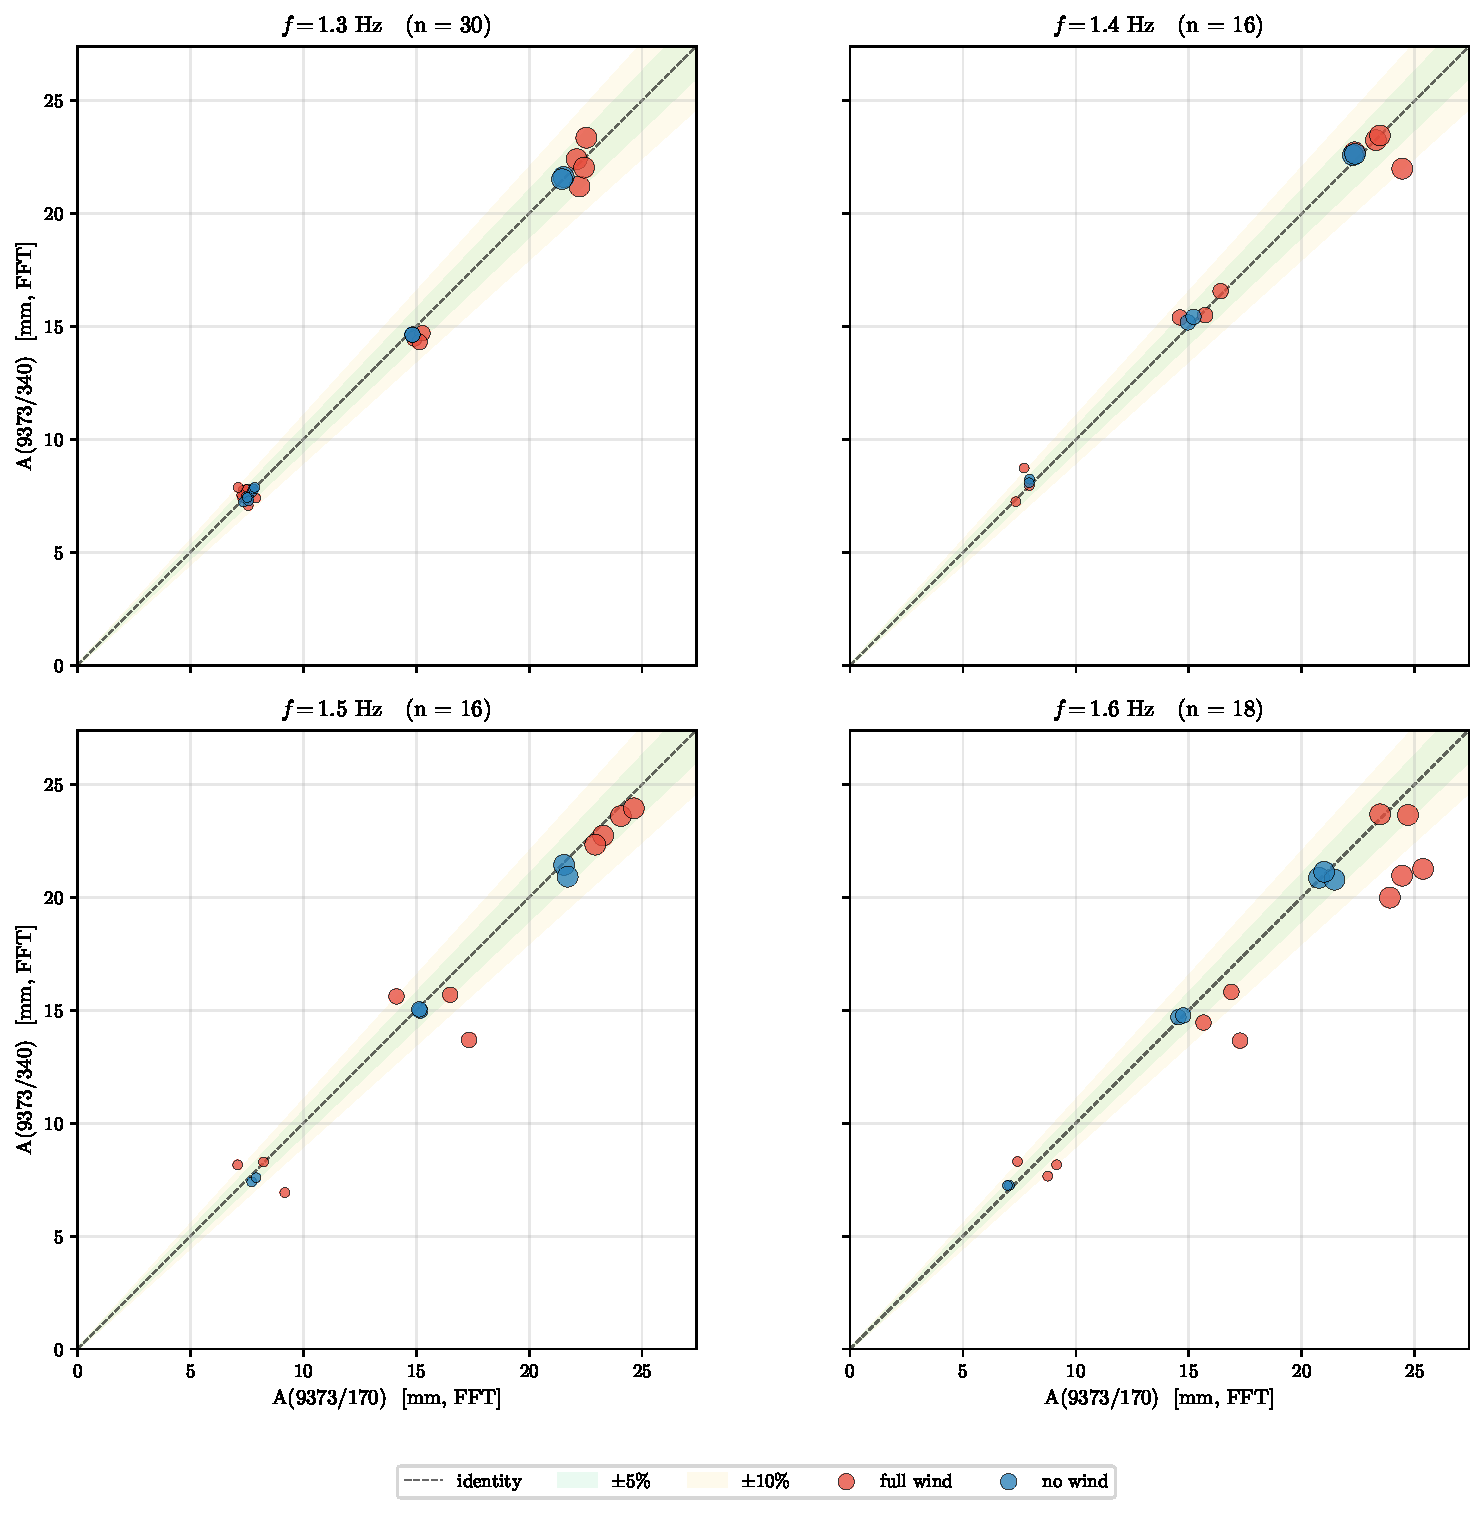
\includegraphics[width=\linewidth]{FIGURES/ch04_parallel_probe_agreement_by_freq.pdf}
  \caption{
    % TODO: write caption
  }
  \label{fig:ch04_parallel_probe_agreement_by_freq}
\end{figure}
